% !TeX spellcheck=en_GB
\section{Preliminary}
\subsection{Linear Programming}
A \textit{linear program}(LP) consists of a set of $n$ \textit{variables} and $m$ \textit{linear constraints}. The LP specifies an objective function which maximizes or minimizes a linear combination of the variables and their coefficients, subject to the $m$ constraints. All variables and constraints must be linear and therefore it is not allowed to multiply variables with each other or itself. To formulate precisely:

\begin{alignat*}{3}
\text{max: } &\sum_{i=1}^{n} c_i x_i\\
\text{s.t }  & \sum_{j=1}^{n} a_{ij} x_j \leq b_i && \text{ for } i=1,2,...,m\\
& x_j \geq 0                         && \text{ for } j=1,2,...,n
\end{alignat*}

The variables can be seen as dimensions in a $n$-dimensional coordinate system and the constraints defines a convex feasibility region where the values of the variables satisfies all of the constraints. An extreme point of the region will have a specific objective value and it can be shown that the optimal value of the linear program can be found in such a point.

\begin{figure}[H]
	\centering
	\label{key}
	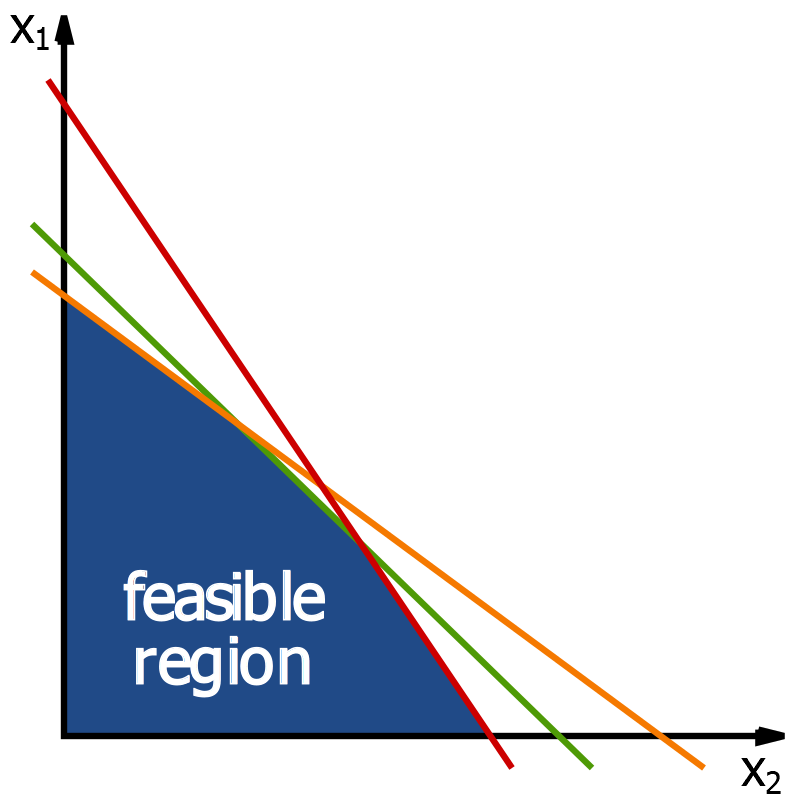
\includegraphics[width=0.6\textwidth]{Linear_Programming_Feasible_Region}
	\caption{My caption}
	\graphicspath{dir-list}
\end{figure}
\todo[inline]{Taget fra wiki så lav vores egen}

The result of running a linear program can either be a vector of the variables of the optimal solution or a scalar representing the resulting value of the objective function depending on what is wanted. Since there can be multiple optimal points the variable vector might be difficult to compare with an expected vector therefore the objective value is often used instead. By adding the constraint that the variables have to be integers the linear programming problem becomes NP-hard. This version is called \textit{Integer Linear Programming} (ILP) and can be used to solve other NP-hard problems quite efficiently. This project does not work dive into ILPs but still have relevance since simplex is also used to solve ILPs by relaxation.

\subsubsection{Simplex}
Simplex is a specific algorithm for solving linear programs. It finds the optimal solution by traversing the extreme points of the feasible region, continuously increasing the objective value.
simplex initiates by generating the \textit{slack formulation} of the LP. To convert LP into slack form first $m$ \textit{slack variables} are introduced as follows.

\begin{alignat*}{3}
\text{max: } &\sum_{i=1}^{n} c_i x_i\\
\text{s.t }  & \sum_{j=1}^{n} a_{ij} x_j + x_{n+i} = b_i  && \text{ for } i=1,2,...,m\\
& x_j \geq 0                                    && \text{ for } j=1,2,...,n+m
\end{alignat*}

Then the slack formulation is achieved by isolating the slack variables in the constraints and changing the maximization to an equality with an unknown constant $z$. In this formulation every variable in the $z$-row is called the \textit{non-basic} variables and the isolated variables in the constraints are called the \textit{basic} variables. Every non-basic variable always has value 0, and every non-basic variable is therefore equal to the constant of the corresponding constraint. The formulation is as follows:

\begin{alignat*}{4}
z        &= && \sum_{i=1}^{n} c_ix_i\\
x_{n+i}  &= && b_i - \sum_{j=1}^{n} a_{ij} x_j  &&& \text{ for } i=1,2,...,m
\end{alignat*}

Given the slack form simplex iteratively pivots variables to increase the objective value. In a pivot a non-basic variable essentially swaps position with a basic variable such that the value of the previously non-basic variable increases until the constraint is tight and the previously basic variable becomes $0$. After the pivot $z$ must either increase stay the same. The variable chosen to leave the non-basic variable is based on picking only variables with positive coefficients. The variable chosen to leave the basic variables is based on which constraint is the most binding, that is the constraint which allows the non-basic variable to increase the least. When it is not possible to pivot any variables without decreasing $z$, that is every coefficient of the non-basic variables are negative, the optimal solution has been found. The solution to the original problem is the set of variables, where every non-basic variable is $0$ and the basic variables are equal to the corresponding constant.


\subsubsection{Representation}
One way to represent the constraints and variables is with vectors and matrices. Since we have a $n$ variables the coefficients of the variables can be encoded in a vector $c$, there are $m$ constants of the constraints which can be encoded into a vector $b$ and the constraints can be seen as a matrix $A$ over every variable and constraint row. The sequential simplex algorithm which functions as the basis for the implementations is based on a compact version of the algorithm presented in [Cormin chapter 21]\todo{proper ref}. The algorithm uses the matrix representation of the linear program.
